\title{Physics 134 
\partition\
Physics Advanced Laboratory\\
\vspace{1ex}
Measurement and Analysis X-Ray Powder Diffractions}
\author{\large Rick Ramirez}
\date{Spring 2016}
\documentclass[12pt]{article}
\usepackage[margin=0.8in]{geometry}
\usepackage{amsmath, amssymb, enumerate, gensymb, wrapfig} %amssymb provides symbols for (integers, reals etc.)
\usepackage{verbatim} % Comment block.
\usepackage{pgfplots} % 3D plots
\pgfplotsset{compat=1.8}
\usepackage{mathrsfs} % provides cursive letters
\usepackage{caption}
\usepackage{booktabs}
\linespread{1.3}
\newcommand{\partition}{\rule{\linewidth}{0.8pt}}

% my own titles
\makeatletter
\renewcommand{\maketitle}{
\begin{center}
\@date \hfill  \@author\\
{\Large \textsc{\@title}}
\partition\\
\end{center}
}
\usepackage{tikz}

%%%----------%%%----------%%%----------%%%----------%%%----------%%%
%%%----------%%%----------%%%----------%%%----------%%%----------%%%

\begin{document}
\maketitle
\linespread{1.5}
\section{Introduction}
\noindent
This experiment utilized X-ray diffraction as a means of studying the structure of 5 materials. When momochromatic X-rays are incident on a crystal at an angle satisfying Braggs 's law, they are diffracted in a particular direction. The pattern produced can be used to study the regular arrangement of the atoms with the material. This is possible because constructive interference occurs only when $\theta_{\text{in}} = \theta_{\text{out}}$,  incident and outgoing rays are coplanar with the normal to the lattice plane, and $E_{\text{in}} = E_{\text{out}}$.
\begin{figure}[h!]\centering
 \quad 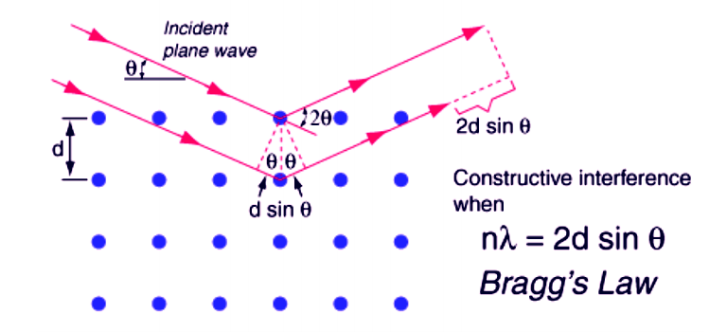
\includegraphics[width=0.6\textwidth]{bragg}
\caption{Braggs Law diagram. Taken from \cite{manual}.}
\label{fig:bragg}
\end{figure} 

\noindent
Figure \ref{fig:bragg} encompasses the simplest case of x-rays on a single crystal lattice. However, this experiment instead uses powder diffraction. Ideally, the tiny crystals of the powder are randomly oriented such that when the constructive interference conditions are met, a series of diffraction cones are produced. The effect is as if the outgoing rays in Fig\ref{fig:bragg} are rotated out of the page to form a complete circle. 

\section{Experimental Setup}
The wavelength of the radiation used in this experiment is on the order of the angstrom $(\AA)$. Consider the Bohr radius; it is the most probable distance between a proton and an electron in the ground state of hydrogen, and is roughly $5.3\times 10^{-11}$ m. The angstrom is  $10^{-10}$ m. Because the distance between two hydrogen nuclei is just over $0.5\AA$, the angstrom is a suitable wavelength to resolve the structure of much larger crystal lattices. 
\subsection{Diffractometer}

The main diffractometer used for this experiment is the Rigaku miniflex. A schematic for the machine can be seen in Fig. \ref{fig:miniflex}. The main components consist of an x-ray generator, focused via a collimeter, a gonimeter (rotating sample holder), and a detector made of a NaI crystal scintillator. 

\begin{figure}[h!]\centering
 \quad 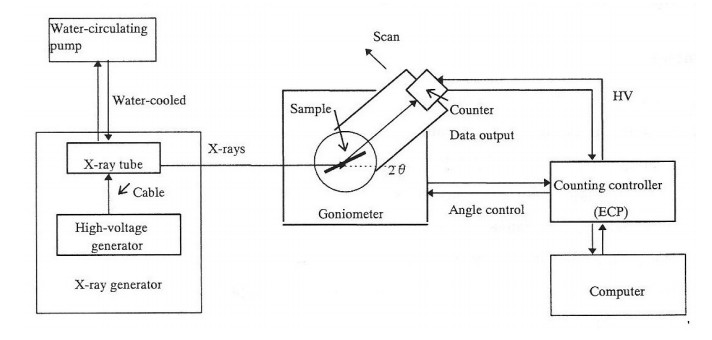
\includegraphics[width=0.6\textwidth]{miniflex}
\caption{Schematic of the Rigaku Miniflex. Taken from  \cite{manual}.}
\label{fig:miniflex}
\end{figure} 

\noindent
Radiation is generated by subjecting the x-ray tube to a high voltage of 30KV. At one end is a tungsten filament that when heated, emits electrons. The electrons are accelerated by the high voltage until they meet a copper anode. When an incoming electron is incident on a copper atom, it eject electrons from the K-shell, causing electrons from the L and M shells to fall and fill the void. The transition of the L electron results in the emission of x-rays with wavelength $1.54059\AA$ (k$\alpha_1$) or $1.5441\AA$ (k$\alpha_2$) depending on spin orientation, while the M electron produces $1.39225\AA$ (k$\beta$) x-rays.

\subsection{X-ray Selection}

Powder diffraction requires the radiation to be monochromatic, so we select only one of the wavelengths produced by the x-ray generator. This is accomplished by either using a k$\beta$-filter to absorb wavelengths below a certain value, or a monochromator. The monochromator ensures that only waves satisfying the bragg condition are diffracted. The rugaku miniflex uses a nickle k$\beta$-filter , while the rigaku smartlab utilizes a molybdenum monochromator.
\section{Procedure}

\subsection{Sample Preparation}
Each of the 5 samples was ground down to as fine a powder as possible. Because the diffractometer's gonimeter is a rotating platform that can also tilt the samples independently, each of the aluminum sample holders was covered with a thin layer of vaseline. This ensures that the samples do not slide off of the stage. The machine's detector was allowed to revolve through an angle of $10\degree$ to an angle of $85\degree$ about the platform.

\begin{figure}[h!]\centering
 \quad 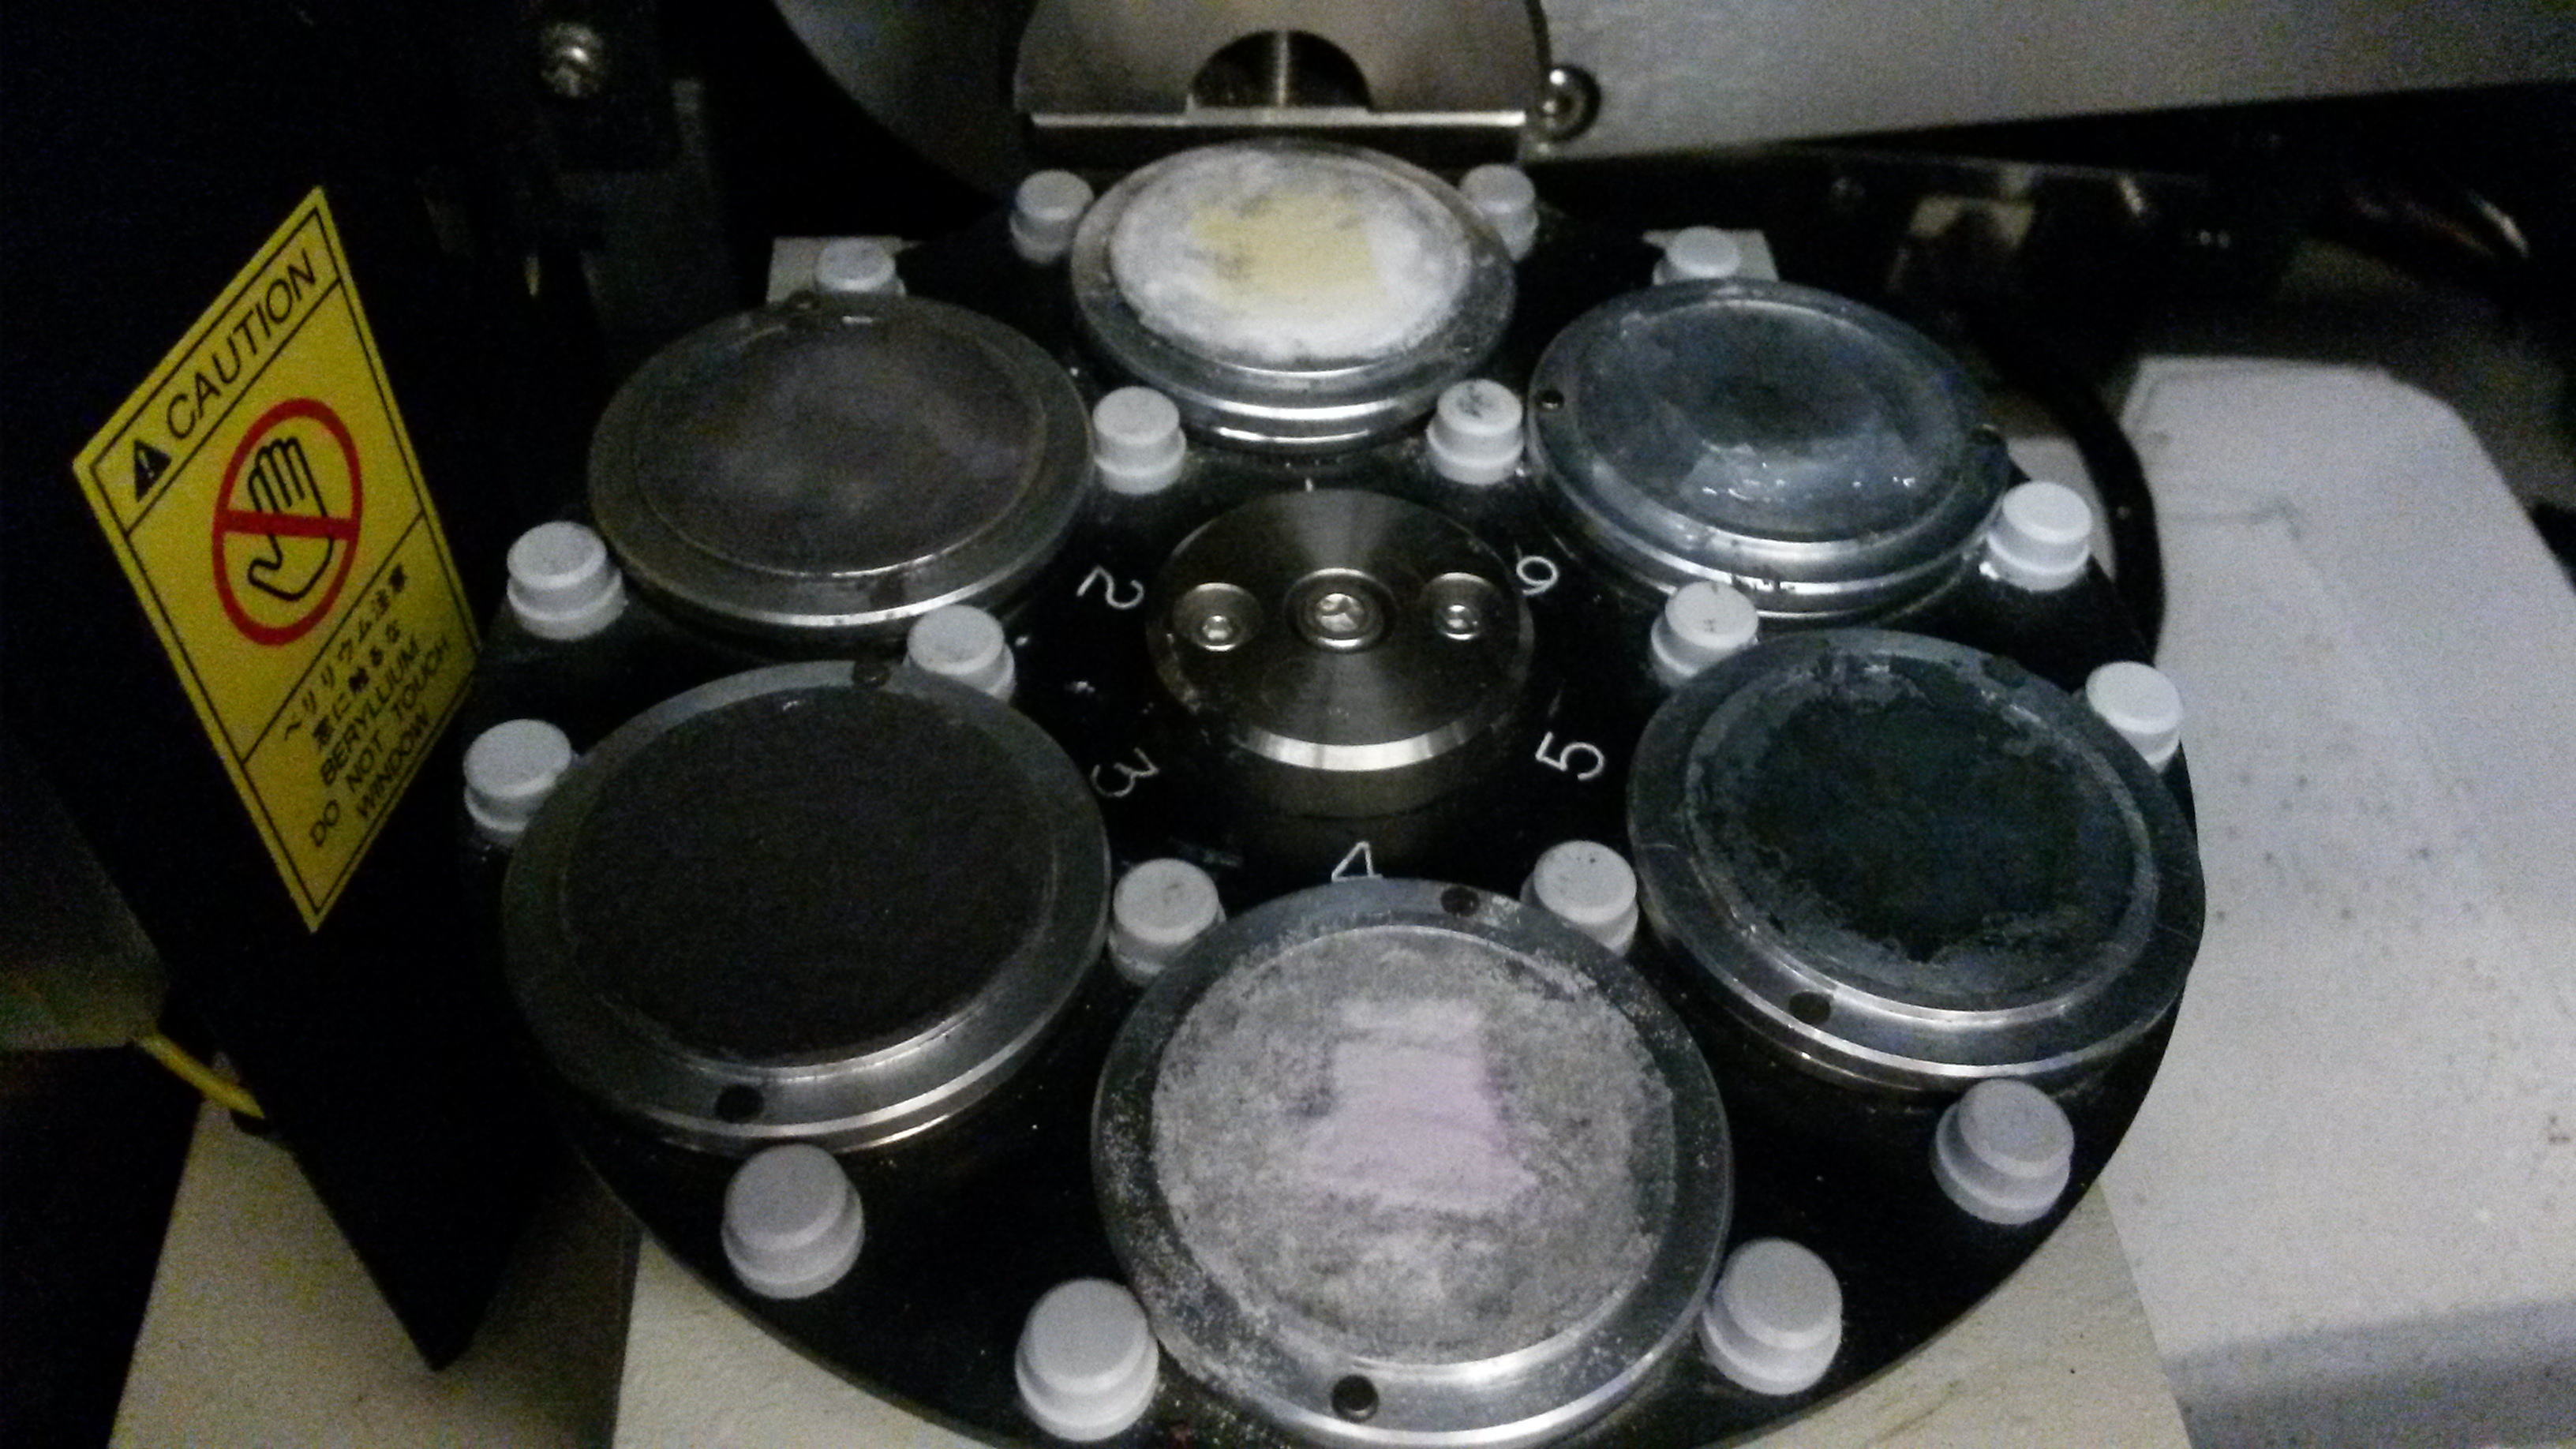
\includegraphics[width=0.8\textwidth]{samples}
\caption{Samples analyzed using the Rigaku miniflex.}
\label{fig:samples}
\end{figure}

\subsection{Refinement}
Data produced by the diffractometer comes in the form of a text file. The file consists of intensity values across across $75\degree$ in steps of $2\theta = 0.02\degree$. When the file is loaded into the program FULLPROF to be refined, all necessary parameters must be initialize. The parameters consist of basis atom locations, space groups, and unit cell occupancies, which are determined by using crystallographic information files from the inorganic crystal structures database. The program utilizes a rietveld refinement method to fit the data to a specified polynomial. This is accomplished by using a least square approach to match the line profile $y_{calc}$ with the measured profile $y_{obs}$ such the the function \cite{Rietveld}
\begin{equation}
M = \sum_i = W_i\left[ y_i^{obs} - \frac{1}{c}y_i^{calc} \right]^2\:,
\end{equation} 
is minimized; where $W_i$ is the weight of each term, and $c$ is an overall scale factor. The shape of the peaks depend on the type of diffraction used. For example, neutron diffraction peaks follow a nearly perfect Gaussian, while x-ray diffraction is best approximated with the summation of Lorentzian and Gaussian functions with adjustable parameters. The width of each peak is dependent on the Bragg angle $2\theta$, and is described in terms of full width half maximum function
\begin{equation}
(\text{FWHM})_k = \text{U}\tan^2\theta_k + \text{V}\tan\theta_k + \text{W}\:,
\end{equation}
where U, V and W are adjustable. The final parameter allowed to vary is the atomic isotropic temperature parameter $B$, which measures how far the atoms move from their normal position. This effect can be minimized by cooling the crystal appropriately (eg. liquid nitrogen).

\noindent
Because the least square method contains too many variables to refine at one time, the process is broken into the following stages:
\begin{itemize}
\item Vary the scale factor, background polynomial, and instrumental zero, with all other parameters held constant
\item Allow the lattice parameters a, b, and c to vary until converged, then set them to fixed.
\item Refine the B factor. 
\item Vary half-width parameters U, V and W one at a time. 
\item Re-refine the B factor.
\end{itemize}
For particularly complicated diffraction patterns, it is useful to introduce more background polynomial terms incrementally.
\newpage
\section{Analysis}

\subsection{Aluminum with Vaseline}
The first sample analyzed consisted of the sample holder with a thick layer of vaseline smeared on it. A preliminary inspection of the data shows a large broad peak extending from around $10^{\degree}$ to $25^{\degree}$, as shown Fig.\ref{fig: Al_vas_win}. This is the result of the layer of vaseline, while the narrow peaks are characteristic of the aluminum. The initial parameters for the refinement were determined using a crystallographic information file from the ICSD database with code 43423, and a summary of the results can be seen in Table \ref{tab:a}.
\begin{figure}[h!]
 \quad 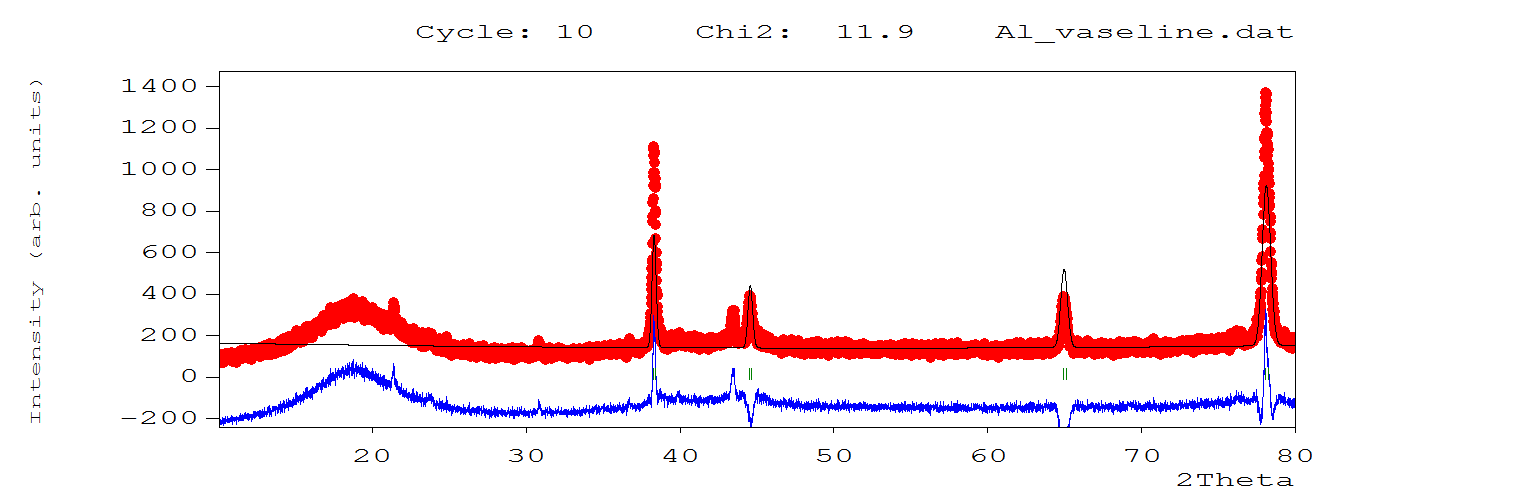
\includegraphics[width=1\textwidth]{vas_peak_refin}
\caption{Plot of aluminum sample holder with vaseline.}
\label{fig: Al_vas_win}
\end{figure}
\begin{table}[htbp]\centering
\begin{tabular}{ |p{3cm}|p{3cm}|}
 \hline
  Space group & \quad F m -3 m\\
 \hline
a = b = c & \quad $4.049(5)\:\AA$\\
\hline
 $\alpha = \beta = \gamma$ & \qquad$90^{\degree}$\\
 \hline
  Rf-factor & \qquad32.9 \\
 \hline
 Bragg R-factor & \qquad 47.2 \\
 \hline
 \qquad\quad $\chi^2$ & \qquad 11.9\\
 \hline
\end{tabular}
\def\sym#1{\ifmmode^{#1}\else\(^{#1}\)\fi}
\caption{Refinement summary of sample holder with vaseline.}\label{tab:a}
\end{table}

\noindent
With this information in mind, a refinement of the data was performed with the region corresponding to the broad vaseline peak excluded, as seen in Fig.\ref{fig: Al_vas_ex}. Table \ref{tab:al_ex} shows that by excluding this region, we greatly improve the value of $\chi^2$. 
\newpage
\begin{figure}[t]
 \quad 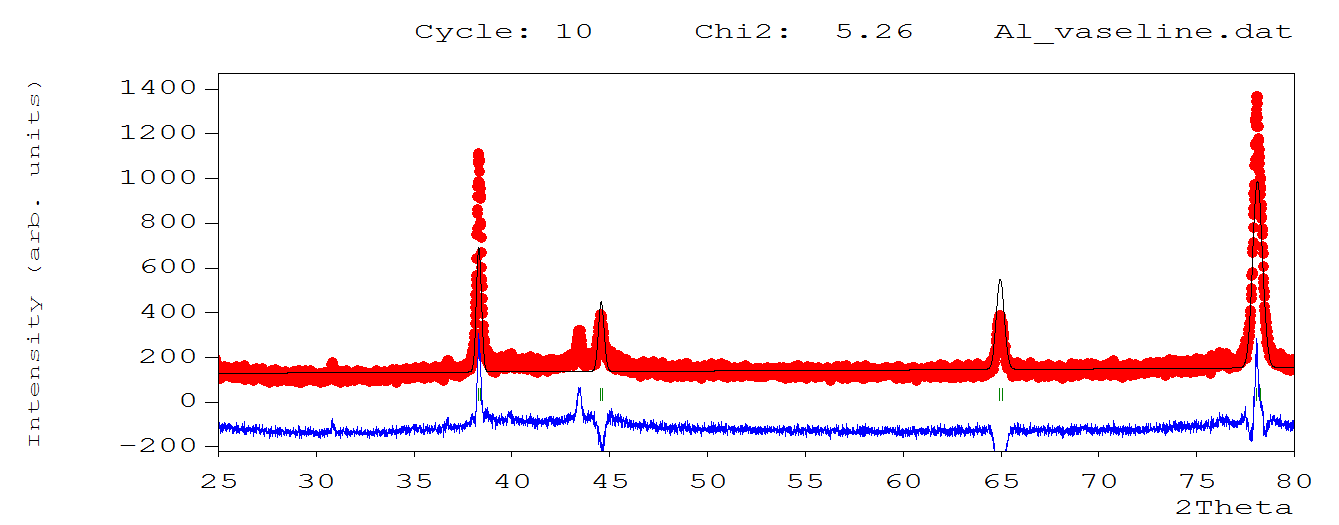
\includegraphics[width=1\textwidth]{al_samp_exclud}
\caption{Plot of aluminum holder with vaseline, excluding the region between $10^{\degree}$ and $25^{\degree}$.}
\label{fig: Al_vas_ex}
\end{figure}

\noindent
With the vaseline region removed, it is clear that aluminum exhibits sharp and widely spaced peaks. This quality in a sample holder is useful because the characteristic peaks of aluminum can easily be removed from the background when examining other materials.\\

\begin{table}[htbp]\centering
\begin{tabular}{ |p{3cm}|p{3cm}|}
 \hline
  Space group & \quad F m -3 m \\
 \hline
a = b = c & \quad $4.049(3)\:\AA$\\
\hline
 $\alpha = \beta = \gamma$ & \qquad$90^{\degree}$\\
 \hline
  Rf-factor & \qquad 36.0\\
 \hline
 Bragg R-factor & \qquad 50.5\\
 \hline
 \qquad\quad $\chi^2$ & \qquad 5.26\\
 \hline
\end{tabular}
\def\sym#1{\ifmmode^{#1}\else\(^{#1}\)\fi}
\caption{Refinement summary of sample holder with vaseline.}\label{tab:al_ex}
\end{table}
\noindent
Figure \ref{fig: Al_vas_ex} also shows that certain peaks are much larger than the predictions of the fitting function. This indicates that the aluminum sample has certain preferred orientations, namely at $2\theta = 38.48\degree$ and $2\theta = 78.25\degree$. The miller indices of these orientations, and for the remaining peaks, are shown in Table \ref{tab:al_miller}. The values of the lattice parameters were found to be 4.049(3) $\AA$, and appears to be in good correspondence to the value of 4.049750(15) $\AA$ as reported in the cif file. Figure \ref{fig: Al_lattice_planes} shows the face-center cubic structure of the aluminum unit cell, as well as the two lattice planes corresponding to the preferred orientations.  \\
\begin{table}[htbp]\centering
\begin{tabular}{ |p{3cm}|p{3cm}|p{3cm}|}
 \hline
  h, k, l & 2$\theta$ ($\degree$)& $d_{hkl}$($\AA$)\\
 \hline
 1 1 1 &  38.48 & 2.34\\
 \hline
 2 0 0 &  44.73 & 2.02\\
 \hline
 2 2 0 &  65.11 & 1.43\\
 \hline
 3 1 1 &  78.25 & 1.22\\
 \hline
\end{tabular}
\def\sym#1{\ifmmode^{#1}\else\(^{#1}\)\fi}
\caption{Miller indices, peak angles, and d-spacing for aluminum provided by FULLPROF.}\label{tab:al_miller}
\end{table}
\begin{figure}[h!]\centering
 \quad 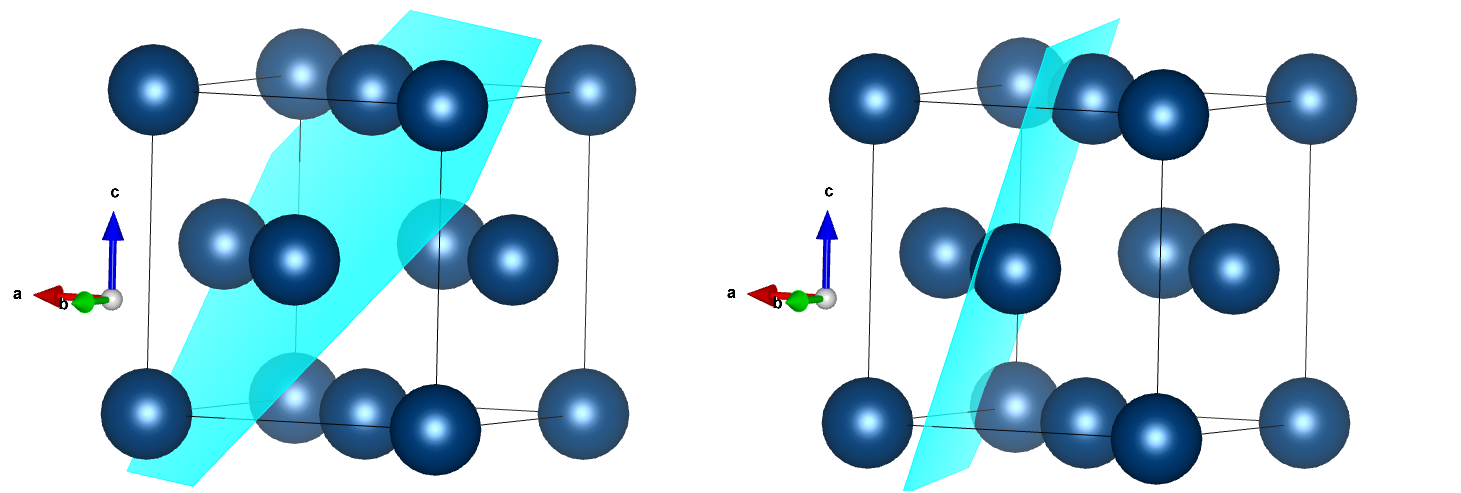
\includegraphics[width=0.8\textwidth]{Al_111Left_311Right}
\caption{FCC structure of aluminum. The lattice plane to the left corresponds to (1, 1, 1) and to the right, (3, 1, 1).}
\label{fig: Al_lattice_planes}
\end{figure}
\subsection{Silicon}
Like aluminum, silicon has a bravais lattice that is face-centered cubic. However as shown in Fig.\ref{fig:Si_structure}, unlike aluminum, silicon exhibits a diamond structure with a space group of F m -3 m:1. The effect of this arrangement is the appearance of four additional basis vectors. In total, the basis consists of \cite{streetman}
\begin{equation*}
\begin{split}
& \vec{a}_0 = 0\hat{x} + 0\hat{y} + 0\hat{z}, \quad \vec{a}_1 = \frac{a}{2}(\hat{x} + \hat{y}), \quad \vec{a}_2 = \frac{a}{2}(\hat{y} + \hat{x}), \quad \vec{a}_3 = \frac{a}{2}(\hat{x} + \hat{z}) \qquad\text(FCC)
\\[1ex]
& \vec{a}_4 = \frac{a}{4}(\hat{x} + \hat{y} + \hat{z}), \quad \vec{a}_4 = \frac{a}{4}(3\hat{x} + 3\hat{y} + \hat{z}), \quad \vec{a}_4 = \frac{a}{4}(\hat{x} + 3\hat{y} + 3\hat{z}), \quad\text{and}\quad \vec{a}_4 = \frac{a}{4}(3\hat{x} + \hat{y} + 3\hat{z})\:,
\end{split}
\end{equation*}
and can be used to calculate the structure amplitude 
\begin{equation}
\textbf{F}_{hkl} = \sum_j\sum_m = f_j \exp(-i\textbf{K}_{hkl} \cdot \textbf{r}_{jm})\:.
\end{equation}
$f_j$ is the structure factor (characteristic of the material), $\textbf{K}_{hkl} = \frac{2\pi}{a}(h\hat{x} + k\hat{y} + l\hat{z})$ is the reciprocal lattice vector for an arbitrary $\left\{h, k, l\right\}$, and $\textbf{r}_{jm}$ is the position of the basis atoms. Carrying out the dot product and summations, we arrive at
\begin{equation}\label{eq:F}
\textbf{F}_{hkl} = f_{Si}\left\{ 1+ e^{-i\pi(k+l)} + e^{-i\pi(h+l)} + e^{-i\pi(h+k)} \right\}\left\{ 1 + e^{-i\frac{\pi}{2}(h+k+l)} \right\}\:.
\end{equation}
The first term on the left is that of the FCC configuration, while the term on the right is the effect of the diamond contribution. Because the square of the structure amplitude is directly proportional to the intensity of the diffraction peak of a given (h, k, l), by finding the zeros of $\textbf{F}_{hkl}$, we can produce a set of extinction rules for a particular lattice. By examining Eq(\ref{eq:F}), we find that 
\begin{itemize}
\item if (h, k, l) are all odd and $h+k+l = 4n\pm 1$:\quad $\textbf{F}_{hkl} = 4(1\pm i)\:f_{Si}$
\item if (h, k, l) are all even and $h+k+l = 4n$: \qquad $\textbf{F}_{hkl} = 8\:f_{Si}$
\item if (h, k, l) mix even and odd, or all even with ($h + k + l$) modulo $4 \neq 0$: \quad $\textbf{F}_{hkl} = 0$
\end{itemize}
Because $I_{hkl}\propto |F_{hkl}|^2$, the allowed reflections should have relative intensities of 64, 32 or 0.\\

\noindent
Two samples of silicon were analyzed with the Rigaku miniflex, with one of the samples ground much finer than the other. The results of the refinement are summarized in Table \ref{tab:Si}, and a plot can be seen in Fig.\ref{fig: groundSi}. The miller indices, along with the corresponding angles, are summarized in Table \ref{tab:Si_miller}. From Fig.\ref{fig: groundSi}, there is a missing peak located at $2\theta = 58.83 \degree$. This corresponds to  miller indices (2 2 2), that produce a sum that is not a multiple of 4, and is expected to cancel according to the extinction rules. 
\begin{figure}[htbp]
 \quad 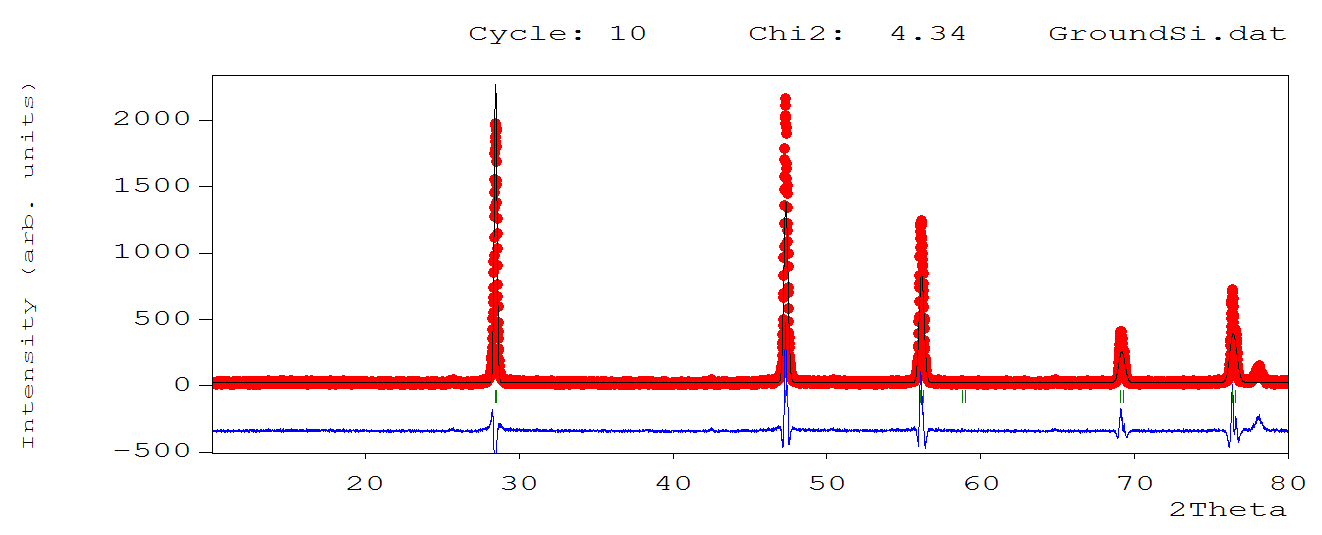
\includegraphics[width=1\textwidth]{gdSi}
\caption{Refinement plot of silicon. Note the missing peak at $2\theta = 58.83\degree$}
\label{fig: groundSi}
\end{figure}

\newpage

\begin{table}[h]\centering
\begin{tabular}{ |p{3cm}|p{3cm}|}
 \hline
  Space group & \quad F m -3 m:1\\
 \hline
a = b = c & \quad $ 5.43(2)\:\AA$\\
\hline
 $\alpha = \beta = \gamma$ & \qquad$90^{\degree}$\\
 \hline
  Rf-factor & \qquad 8.24 \\
 \hline
 Bragg R-factor & \qquad 15.2 \\
 \hline
 \qquad\quad $\chi^2$ & \qquad 4.34\\
 \hline
\end{tabular}
\def\sym#1{\ifmmode^{#1}\else\(^{#1}\)\fi}
\caption{Refinement summary of silicon.}\label{tab:Si}
\end{table}

\setlength{\belowdisplayskip}{1pt} \setlength{\belowdisplayshortskip}{1pt}
\setlength{\abovedisplayskip}{1pt} \setlength{\abovedisplayshortskip}{1pt}


\noindent
The d-spacing values of Table \ref{tab:Si_miller} were calculated using braggs law
\begin{equation}
2d \sin(\theta) = n\lambda\:.
\end{equation}
For a cubic system, these can be used to calculate the length of the unit cell by
\begin{equation}
a = d_{hkl}\sqrt{h^2 + k^2 + l^2}\:.
\end{equation}

\begin{table}[h!]\centering
\begin{tabular}{ |p{3cm}|p{3cm}|p{3cm}|}
 \hline
  h, k, l & 2$\theta$ ($\degree$)& $d_{hkl}$($\AA$)\\
 \hline
 1 1 1 &  28.43 & 3.14\\
 \hline
 2 2 0 &  47.29 & 1.92\\
 \hline
 3 1 1 &  56.10 & 1.64\\
 \hline
 2 2 2 &  58.83 & 1.57\\
 \hline
 4 0 0 &  69.01 & 1.36\\
 \hline
 3 3 1 &  76.35 & 1.24\\
 \hline
\end{tabular}
\def\sym#1{\ifmmode^{#1}\else\(^{#1}\)\fi}
\caption{Miller indices, peak angles, and d-spacing for silicon.}\label{tab:Si_miller}
\end{table}
 

\begin{figure}[h!]\centering
 \quad 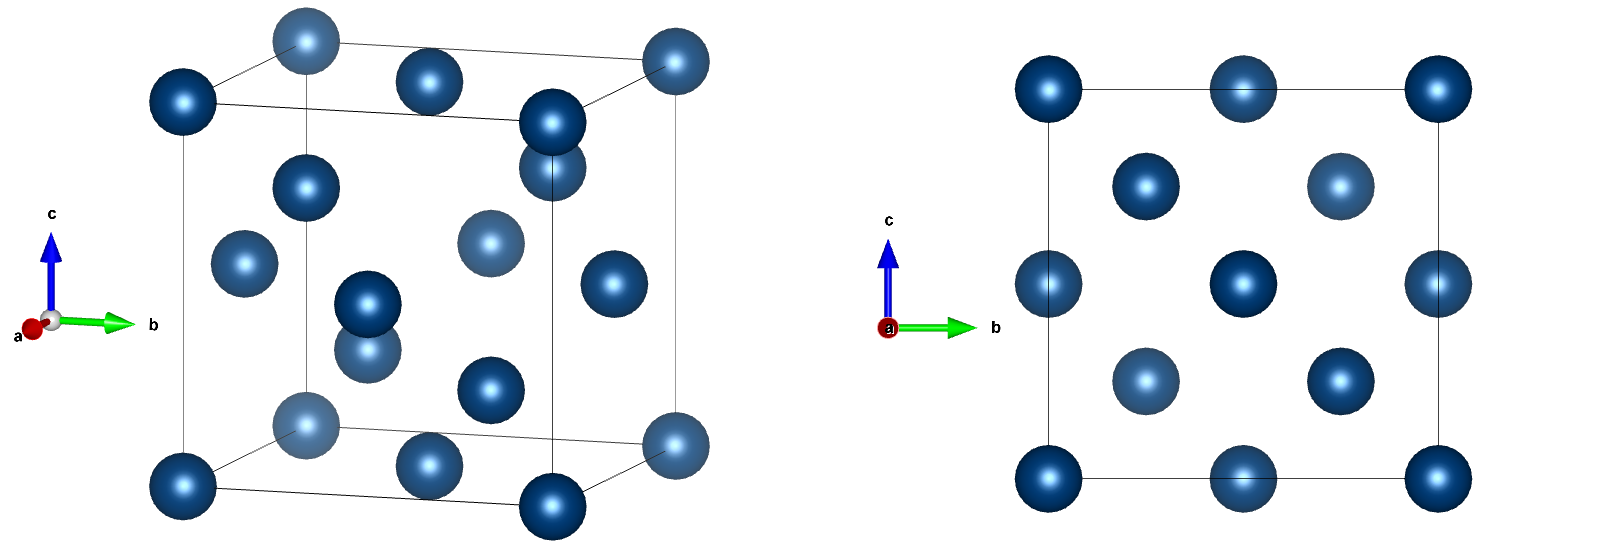
\includegraphics[width=0.7\textwidth]{Si_structure}
\caption{Diamond structure of silicon.}
\label{fig:Si_structure}
\end{figure}

\noindent
A calculation of the unit cell length produces produces a value of $5.43 \: \AA$ and agrees with the value produced by FULLPROF and reported by ICSD.

\newpage
\subsection{Sodium Chloride}
The next sample analyzed was sodium chloride. It has a space group of Fm-3m with each of the two species of atoms forming separate, but overlapping, face center cubic lattices as shown in Fig.\ref{fig:NaCl_struct}. 
\begin{figure}[h!]\centering
 \quad 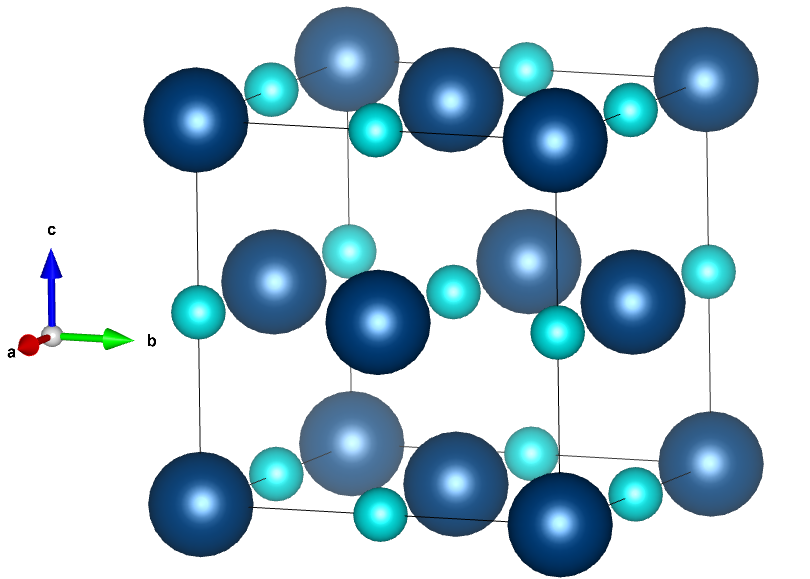
\includegraphics[width=0.4\textwidth]{Nacl_struct}
\caption{Unit cell of sodium chloride.}
\label{fig:NaCl_struct}
\end{figure}

\noindent
Following the same procedure as for silicon, the NaCl structure amplitude  simplifies to

\begin{equation}
\textbf{F}_{hkl} = \left[ f_{\text{Na}^+} + f_{\text{Cl}^-}e^{i\pi (h+k+l)} \right]\left[1 + e^{i\pi (h+k)} + e^{i\pi (k+l)} + e^{i\pi (h+l) } \right]\:,
\end{equation}\\
\noindent
to produce the extinction rules:

\begin{itemize}
\item if (h k l) mix even and odd: $\textbf{F}_{hkl}=0$
\item if (h k l) are homogeneous:
\begin{itemize}
\item[\textbullet] with $(h + k + l)$ even: $\textbf{F}^2_{hkl}=16\left[ f_{\text{Na}^+} + f_{\text{Cl}^-} \right]^2$\\
\item[\textbullet] with $(h + k + l)$ odd: $\textbf{F}^2_{hkl}=16\left[ f_{\text{Na}^+} - f_{\text{Cl}^-} \right]^2$
\end{itemize}
\vspace{5mm} 
 

\noindent
A comparison of the extinction rules with the miller indices in Table \ref{tab:NaCl_miller} indicates that none of the peaks should exhibit cancellation.  Figure \ref{fig:NaCl_refinement} shows a plot of the refinement with some of the peaks appearing nearly flat. The low intensity of these locations correspond to miller indides that consist of all odd values. If the electron configuration of $\text{Na}^+$ and $\text{Cl}^-$ were equal, there would be a complete cancellation. The sample assumes a preferred orientation at $2\theta = 31.66\degree$. The results of the refinement can be seen in Table \ref{tab:Nacl} with a calculated value of $5.64(3)\:\AA$ for the unit cell length.
\end{itemize}

\newpage
\begin{figure}[h!]
 \quad 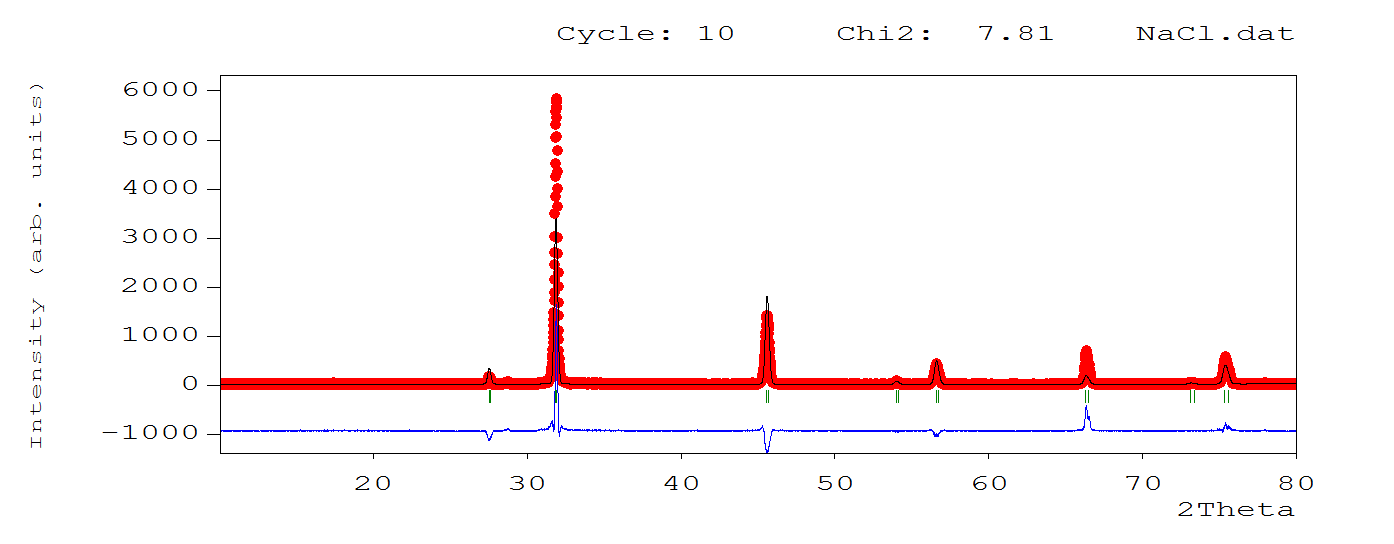
\includegraphics[width=1\textwidth]{NaCl_refinement}
\caption{FULLPROF refinement of NaCl.}
\label{fig:NaCl_refinement}
\end{figure}
\begin{table}[h!]\centering
\begin{tabular}{ |p{3cm}|p{3cm}|}
 \hline
  Space group & \quad F m -3 m\\
 \hline
a = b = c & \quad $5.64(3)\:\AA$\\
\hline
 $\alpha = \beta = \gamma$ & \qquad $90^{\degree}$\\
 \hline
  Rf-factor & \qquad 22.6 \\
 \hline
 Bragg R-factor & \qquad 35.6 \\
 \hline
 \qquad\quad $\chi^2$ & \qquad 7.81\\
 \hline
\end{tabular}
\def\sym#1{\ifmmode^{#1}\else\(^{#1}\)\fi}
\caption{Refinement summary of sodium chloride.}\label{tab:Nacl}
\end{table}

\noindent
It should be noted that the photo in Fig.\ref{fig:samples} was taken after the samples were subjected to radiation. Initially, the NaCl sample (position 1) was pure white, but changed colors during the procedure. This effect is the result of Farbe centers forming within the sample. \cite{West} When NaCl is subjected to ionizing radiation, certain atoms are displaced from their crystallographic position creating vacancies to be filled with electrons. The scenario is essentially an electron in a box with a series of available transitions coinciding with the visible spectrum. The result is that a material that would otherwise be transparent becomes colored. 

\begin{table}[h!]\centering
\begin{tabular}{ |p{3cm}|p{3cm}|p{3cm}|}
 \hline
  h, k, l & 2$\theta$ ($\degree$)& $d_{hkl}$($\AA$)\\
 \hline
 1 1 1 &  27.33 & 3.26\\
 \hline
 2 0 0 &  31.66 & 2.82\\
 \hline
 2 2 0 &  45.38 & 1.99\\
 \hline
 3 1 1 &  53.79 & 1.70\\
 \hline
 2 2 2 &  56.38 & 0.63\\
 \hline
 4 0 0 &  66.12 & 1.41\\
 \hline
 3 3 1 &  72.95 & 1.30\\
 \hline
 4 2 0 &  75.17 & 1.26\\
 \hline
\end{tabular}
\def\sym#1{\ifmmode^{#1}\else\(^{#1}\)\fi}
\caption{Miller indices, peak angles, and d-spacing for sodium chloride.}\label{tab:NaCl_miller}
\end{table}



\newpage
\subsection{Cobalt (II, III) Oxide}
Refinement of cobalt oxide data, taken from the Rigaku miniflex, produces results that are unlike any of the other samples Fig.\ref{fig:co3o4}.  The nickle K$\beta$-filters used by this diffractometer have a K-adsorption edge of $\lambda = 1.488\AA$; that is, higher energy photons with wavelengths bellow this value are absorbed. Nickle effectively absorbs the K$\beta$ radiation of the copper anode, and only allows K$\alpha$ ($\lambda = 1.54\AA$) to pass through. The absorption edge of cobalt lies at $\lambda = 1.608\AA$, only slightly above the wavelength of the K$\alpha$. As a result, the cobalt sample absorbs the K$\alpha$ radiation causing the material to fluoresce. This produces the unusually broad background in Fig.\ref{fig:co3o4}.
\begin{figure}[h!]
 \quad 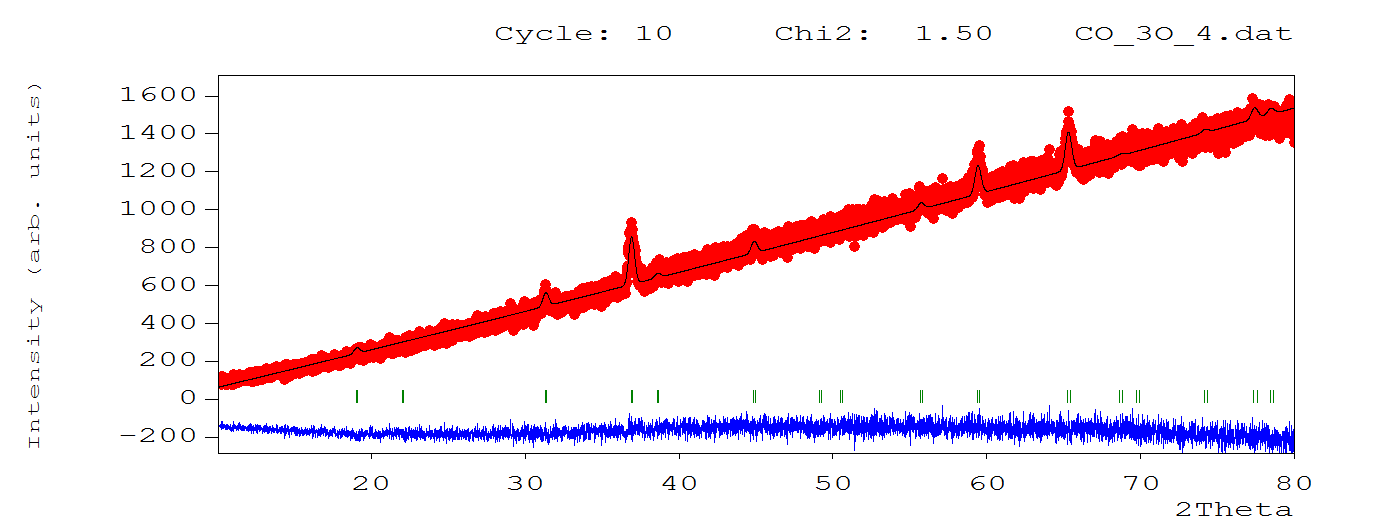
\includegraphics[width=1\textwidth]{Co3O4_refinement}
\caption{Refinement plot of Cobalt (II, III) Oxide using Rigaku Miniflex}
\label{fig:co3o4}
\end{figure}

\newpage
\noindent
To remedy this effect, a separate diffractometer (Rigaku Smartlab), with monochromators placed between the sample and the detector, was used. This allows only x-rays satisfying bragg's law to diffract. The results of using this apparatus can be seen in Fig.\ref{fig:co3o4_smart} and Table \ref{tab:co3o4}.
\begin{figure}[h!]
 \quad 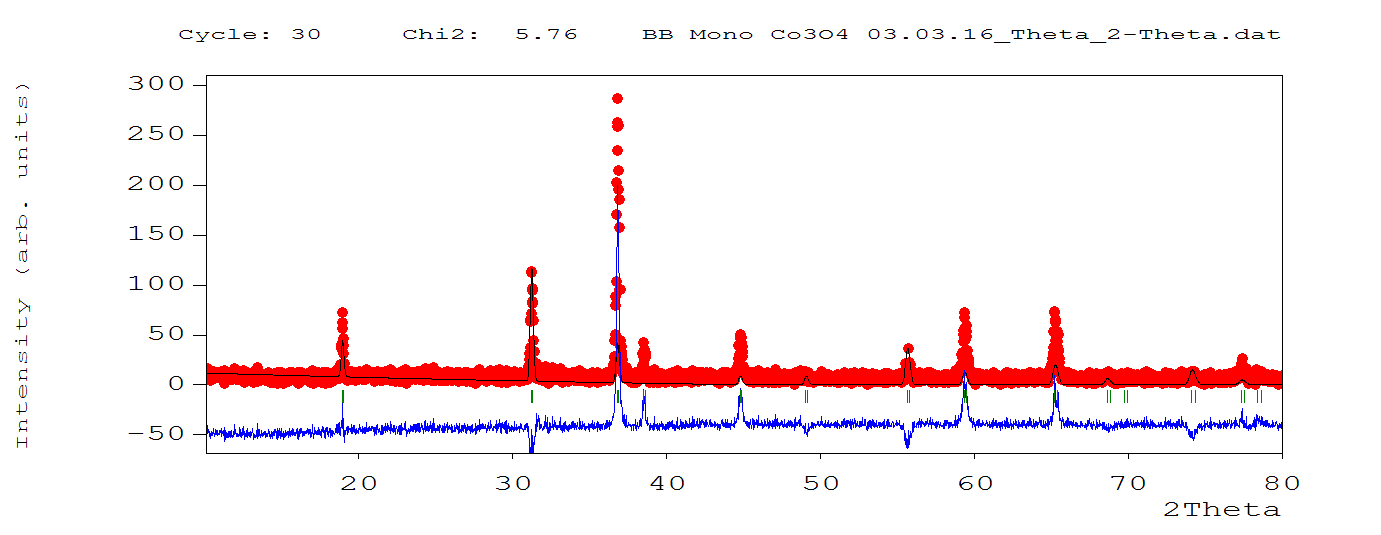
\includegraphics[width=1\textwidth]{co3o4_smart}
\caption{Refinement plot of Cobalt (II, III) Oxide using data from Rigaku Smartlab.}
\label{fig:co3o4_smart}
\end{figure}

\begin{table}[h!]\centering
\begin{tabular}{ |p{3cm}|p{3cm}|}
 \hline
  Space group & \quad F d 3 m\\
 \hline
a = b = c & \quad $8.057(9)\:\AA$\\
\hline
 $\alpha = \beta = \gamma$ & \qquad $90^{\degree}$\\
 \hline
  Rf-factor & \qquad 54.9 \\
 \hline
 Bragg R-factor & \qquad 65.5 \\
 \hline
 \qquad\quad $\chi^2$ & \qquad 6.48 \\
 \hline
\end{tabular}
\def\sym#1{\ifmmode^{#1}\else\(^{#1}\)\fi}
\caption{Refinement summary of Co3O4.}\label{tab:co3o4}
\end{table}

\begin{figure}[h!]\centering
 \quad 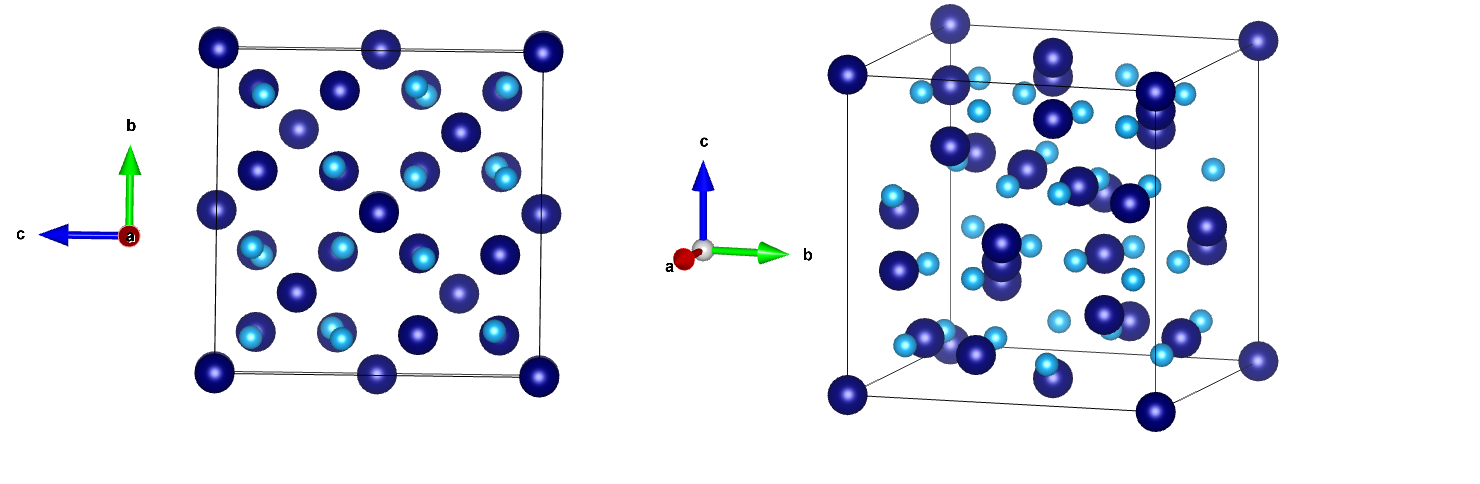
\includegraphics[width=0.8\textwidth]{co3o4_struct_2}
\caption{Structure of Cobalt (II, III) Oxide.}
\label{fig:co3o4_struct_2}
\end{figure}

\newpage

\begin{table}[t]\centering
\begin{tabular}{ |p{3cm}|p{3cm}|p{3cm}|}
 \hline
  h, k, l & 2$\theta$ ($\degree$)& $d_{hkl}$($\AA$)\\
 \hline
 1 1 1 &  19.06 & 4.65\\
 \hline
 2 0 0 &  22.04 & 4.03\\
 \hline
 2 2 0 &  31.37 & 2.85\\
 \hline
 3 1 1 &  36.97 & 2.43\\
 \hline
 2 2 2 &  38.68 & 2.32\\
 \hline
 4 0 0 &  44.96 & 2.01\\
 \hline
 3 3 1 &  49.25 & 1.85\\
 \hline
 4 2 0 &  50.62 & 1.80\\
 \hline
 4 2 2 &  55.85 & 1.64\\
 \hline
 3 3 3 &  59.57 & 1.55\\
 \hline
 5 1 1 &  59.57 & 1.55\\
 \hline
 4 4 0 &  65.47 & 1.42\\
 \hline
 5 3 1 &  68.88 & 1.36\\
 \hline
 4 4 2 &  69.70 & 1.34\\
 \hline
 6 0 0 &  69.97 & 1.34\\
 \hline
 6 2 0 &  74.40 & 1.27\\
 \hline
 5 3 3 &  77.64 & 1.22\\
 \hline
 5 2 2 &  78.71 & 1.21\\
 \hline
\end{tabular}
\def\sym#1{\ifmmode^{#1}\else\(^{#1}\)\fi}
\caption{Miller indices, peak angles, and d-spacing for sodium chloride.}\label{tab:NaCl_miller}
\end{table}

\subsection{Unknown}
The last sample analyzed was presented as an unknown. The first sign to its chemical makeup comes from Fig.\ref{fig:samples} (position 4). Similar to NaCl, this sample shows faint signs of the formation of Farbe centers. The color formation of the sample, after being placed in the diffractometer, is characteristic of potassium; a light purple hue.  After this sample was refined with each of the previous cif files, it was found that NaCl produced the closest fit. With this information, it was determined that the sample consisted of potassium chloride. The lattice parameter was found to be $6.31(9)\:\AA$. A summary of the refinement can be seen in Table \ref{tab:KCl}. \\\\

\noindent
The extinction rules for KCl are identical to that of NaCl with the atomic scattering factor for Na replaced with K. Figure \ref{fig:unknown} shows that there are peak cancellations at $2\theta = 24.39\degree$, $2\theta = 47.73\degree$, $2\theta = 64.24\degree$, and $2\theta = 78.67\degree$ corresponding to miller indices (1 1 1), (3 1 1), (3 3 1), and \\
(3 3 3)/(5 1 1) respectively. This is to be expected considering that for odd indices, the structure amplitude takes the form
\begin{equation}
\textbf{F}^2_{hkl}=16\left[ f_{\text{K}^+} - f_{\text{Cl}^-} \right]^2\:.
\end{equation}
When the ratio $\frac{\sin\theta}{\lambda} = 0$, the scattering factor is equal to the sum of the electrons for each species of atom. Because $\text{K}^+$ and $\text{Cl}^-$ both have 18 electrons, there is a nearly complete cancellation of these diffraction peaks.


\begin{figure}[h!]\centering
 \quad 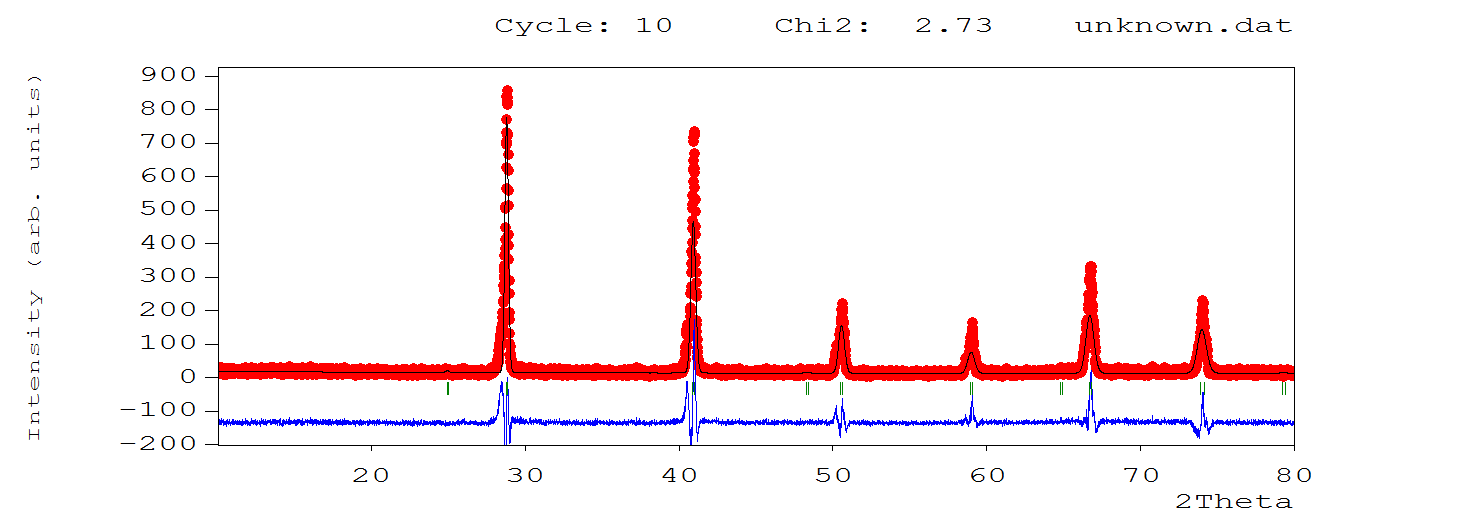
\includegraphics[width=1\textwidth]{unknown}
\caption{Refinement plot of unknown assuming chemical makeup of potassium chloride.}
\label{fig:unknown}
\end{figure}

\begin{table}[h!]\centering
\begin{tabular}{ |p{3cm}|p{3cm}|}
 \hline
  Space group & \quad F m -3 m\\
 \hline
a = b = c & \quad $6.31(9)\:\AA$\\
\hline
 $\alpha = \beta = \gamma$ & \qquad $90^{\degree}$\\
 \hline
  Rf-factor & \qquad 12.9 \\
 \hline
 Bragg R-factor & \qquad 19.6 \\
 \hline
 \qquad\quad $\chi^2$ & \qquad 2.73 \\
 \hline
\end{tabular}
\def\sym#1{\ifmmode^{#1}\else\(^{#1}\)\fi}
\caption{Refinement summary of KCl.}\label{tab:KCl}
\end{table}
\newpage
\begin{table}[h!]\centering
\begin{tabular}{ |p{3cm}|p{3cm}|p{3cm}|}
 \hline
  h, k, l & 2$\theta$ ($\degree$)& $d_{hkl}$($\AA$)\\
 \hline
 1 1 1 &  24.39 & 3.65\\
 \hline
 2 0 0 &  28.24 & 3.16\\
 \hline
 2 2 0 &  40.37 & 2.23\\
 \hline
 3 1 1 &  47.73 & 1.90\\
 \hline
 2 2 2 &  49.99 & 1.82\\
 \hline
 4 0 0 &  58.41 & 1.57\\
 \hline
 3 3 1 &  64.24 & 1.45\\
 \hline
 4 2 0 &  66.12 & 1.41\\
 \hline
 4 2 2 &  73.39 & 1.29\\
 \hline
 3 3 3 &  78.67 & 1.22\\
 \hline
 5 1 1 &  78.67 & 1.22\\
 \hline
\end{tabular}
\def\sym#1{\ifmmode^{#1}\else\(^{#1}\)\fi}
\caption{Miller indices, peak angles, and d-spacing for Unknown.}\label{tab:unknown_miller}
\end{table}

\begin{figure}[h!]\centering
 \quad 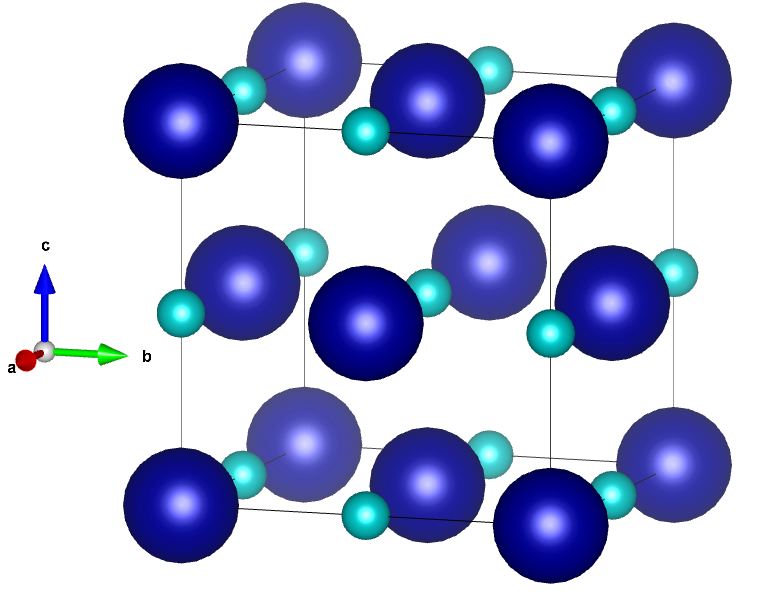
\includegraphics[width=0.3\textwidth]{kcl_struct}
\caption{Structure of potassium chloride.}
\label{fig:kcl_struct}
\end{figure}


\section{Conclusion}
By subjecting powder samples to high energy x-rays to produce diffraction patterns, we were able to determine the intensity as a function of the bragg angle, the length of the unit cell, and the underlying structure of 5 specimens. Comparing the result of each refinement with outside sources reveals how powerful the Rietveld method is at approximating the lattice structure of crystals. This is especially true considering that the method was not fully intended to be applied to powder diffraction.









\newpage
\begin{thebibliography}{9}

\bibitem{manual}
Physics 134 Lab Manual. Spring 2016

\bibitem{Rietveld}
H.M. Rietveld.
\textit{A Profile Refinement Method for Nuclear and Magnetic Structures}. Reactor Centrum Nederland, (1968)

\bibitem{streetman}
Ben G. Streetman, Sanjay Banerjee.
\textit{Solid State Electronic Devices (6th Edition)}. Prentice Hall of India, (2005), ISBN-13: 978-8120330207

\bibitem{West}
Anthony R. West.
\textit{Solid State Chemistry and its Applications}. John Wiley\& Sons, (1990),  ISBN-13: 978-1119942948

\bibitem{icsd}
 Inorganic Crystal Structures Database. \textit{https://icsd.fiz-karlsruhe.de/search/index.xhtml}

\end{thebibliography}









\end{document}